\documentclass[usletter,aps,prb,10pt,amssymb,amsmath,twocolumn]{revtex4-1}
%\usepackage{fullpage}
\usepackage{graphicx}
\usepackage{caption}
\usepackage{subcaption}
\usepackage{wrapfig}
%\usepackage{amsmath}
\usepackage{anyfontsize}




\begin{document}
\title{2-D Electronic Spin Susceptibility Enhancement in Pauli Limited Unconventional Superconductors}
\author{Ben Rosemeyer, Anton Vorontsov}
\affiliation{Department of Physics Montana State University}
\date{\today}
\begin{abstract}
We calculate the wave-vector dependent electronic spin susceptibility for wave vectors $\bf q$ which connect points of zero energy excitations for both quasiparticles and normal state electrons ($\epsilon_{{\bf k},s} = \xi_{{\bf k},s} = 0$) with a uniform applied field ${\bf H}_0$ in the superconducting state. We consider Pauli limited materials with D-wave symmetry, and a quasi 2-D electronic spectrum such as seen in the heavy fermion superconductor CeCoIn$_5$. The longitudinal and transverse components are enhanced over their normal state values in the high field low temperature (HFLT) region of the H-T phase diagram. We identify six critical wave vectors which are candidates for enhancement and discuss how they relate to the formula for $\chi^{sc}$. We also consider temperature and field variations for the two wave vectors with magnitude $|q|\approx 2k_f$.

%There are two critical wave vectos $\bf q^*$ which result in a near maximal $\delta\chi_{\alpha}= \chi^{sc}_{\alpha}-\chi^N_{\alpha}$, for $\alpha = \parallel, \perp$ respectively. These wave vectors connect points on the Fermi surface which have zero quasi-particle excitation energy. We discuss how the phase space available for these excitations effects the ideal wave vector at zero and finite temperatures.
\end{abstract}
\maketitle


\section{Introduction}
The interplay of antiferromagnetism (AFM) and superconductivity has challenged our understanding of these two phenomenon~\cite{spin_sus_dyn,sdw_vortex,sc_afm_ikeda,sc_afm_kato,mag_afm_fflo_sigrist,sc_sdw_anton}. Various materials can be doped to achieve a coexistence phase (CITE), while CeCoIn$_5$ manifests a coexistent AFM and superconducting state in the high field low temperature limit. yet other materials have AFM and superconductivity as close neighbors in their phase diagram (CITE). Indeed, these new materials offer an exciting array of possibilities and unanswered questions to physics.

Experimental results for CeCoIn$_5$ indicate that its coexistence phase depends on the presence of superconducting order~\cite{cecoin5_Bianchi,cecoin5_Kenzelmann,cecoin5_Kenzelmann2}. This phase, commonly called the Q-phase, is limited by a first order transition to the normal state at the upper critical field of a Pauli limited superconductor (H$_{c2}$) in which both superconductivity and AFM order are destroyed. The lower transition is of second order, just below H$_{c2}$. The collapse of AFM with superconductivity implies that the magnetically ordered state is dependent on the presense of superconducting order and copper paired electrons. 

Other results for CeCoIn$_5$ show that the magnetic ordering wave vector in the Q-phase displays little or no dependence on field (within experimental error), which indicates a relatively small or non-existent interaction with the flux lattice ~\cite{cecoin5_Kenzelmann2}. This phenomenon has not been directly addressed in many of the current theories. Our findings indicate that this behavior is more consistent with the longitudinal component of susceptibility rather than the transverse. This is another area of study which has not been very thouroghly analyzed.

Many theories have been proposed to explain the experimental results seen in CeCoIn$_5$, including various manifestations of the FFLO state where the superconducting order parameter oscillates in real space. ~\cite{sc_sdw_anton,mag_afm_fflo_sigrist,fflo_pen_depth,sc_afm_kato,sc_afm_ikeda,sdw_vortex}. The FFLO state has long been believed to offer the possibility of magentic order, however, the predicted field dependence of the ordering vector is not seen in experiment, and recent experiments point to a homogeneous gap function  ~\cite{cecoin5_Kenzelmann2, copperPairsCeCoIn5}. 

Yet other theories offer insight but leave many questions unanswered. Such as: How does the ordering wave vector change with applied field? What are the necessary conditions on the order parameter? And what roles do the transverse and longitudinal components of the magnatism play? Here we provide a first principles approach to these problems by calculating the magnetic susceptibility of itinerant electrons in the D-wave superconducting state. 

\begin{figure}
 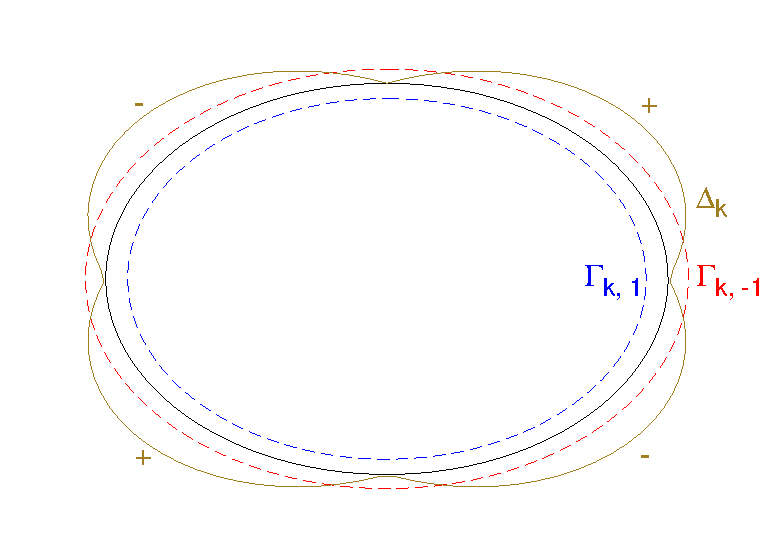
\includegraphics[width = 0.45\textwidth, height = 0.39\textwidth]{./figures/fermi_schematic.eps}
 \caption{we consider a Zeeman split fermi surface ($\Gamma_{k,1}, \Gamma_{k, -1}$) with a $d_{xy}$ symmetric order parameter $\Delta_k=sin(2\theta)$. }
 \end{figure}

\section{Model}
Our model begins with a mean field Hamiltonian which has a 2-D free electron part, a Zeeman part and a superconducting term:

\begin{align*}
\mathcal{H} = \sum_{{\bf k},s} \bigg(\frac{k^2}{2m} - \mu + s\mu_b H\bigg)c_{{\bf k},s}^\dagger c_{{\bf k},s}  \\
- \sum_{\bf k} \Delta_{\bf k} c_{{\bf k},1}^\dagger c_{-{\bf k},-1}^\dagger+\Delta^*_{\bf k} c_{-{\bf k},-1} c_{{\bf k},1}
\end{align*}

From this we can write the electron excitation energies $\xi_{{\bf k}s}=\frac{k^2}{2m^*}+s\mu_b H-\mu$ ($s=\pm1 $), and preform a Bogolioubov transformation which allows us to diagnolize the Hamiltonian (equations 1)~\cite{tinkham}.

\begin{subequations}
\begin{align}
&c^{\dagger}_{{\bf k}, 1}=u_{{\bf k}}\gamma^\dagger_{{\bf k}, -1}+v^*_{{\bf k}}\gamma_{{\bf k}, 1}  \\
&c^{\dagger}_{-{\bf k}, -1}=u_{{\bf k}}\gamma^\dagger_{{\bf k}, 1}-v^*_{{\bf k}}\gamma_{{\bf k}, -1}  \\
&\epsilon_{{\bf k},s}=\sqrt{\Delta_{{\bf k}}^2+\xi_{{\bf k}}^2} + s\mu_e H_z \\
&u_{{\bf k}}=sign(\Delta_{\bf k}) \sqrt{\frac{1}{2}\bigg(1+\frac{\xi_{{\bf k}}}{\sqrt{\Delta_{{\bf k}}^2+\xi_{{\bf k}}^2}}\bigg)} \\
&v_{{\bf k}}^2=1-u_{{\bf k}}^2 
\end{align}
\end{subequations}

we then use the diagnolized Hamiltonian to compute the magnetic susceptibility for electrons in the superconducting state (equations 2, 3)~\cite{mahan}

{\fontsize{5}{0}\selectfont
\begin{align}
\chi_{\alpha\beta}({\bf q})=\mu_e^2\sum\limits_{{\bf k}ss'tt'}\int\limits_0^{\beta}d\tau\sigma^\alpha_{ss'}\sigma^\beta_{tt'}<c^\dagger_{{\bf k+q}, s}(\tau)c_{{\bf k}, s'}(\tau)c^\dagger_{{\bf k+q}, t}(0)c_{{\bf k}, t'}(0)> 
\end{align}
}

Equation 2 describes how the bulk electronic magnetization, $\bf M_{\alpha}$, depends on field:\\
$\bf M_{\alpha}=M_{0,\alpha}({\bf H}_0, {\bf q} = 0)+\chi_{\alpha\beta}({\bf q}) \delta H_\beta$ \\
Here we have used a perterbative approach to the magnetism which is due to a field ${\bf  H = H}_0+\delta{\bf H}$. We consider the perterbative field $\delta{\bf H}<<{\bf H}_0$ to be some small field, which in the case of CeCoIn$_5$, may be due to the localized moments on the Ce atoms.

For electrons in the superconducting state, the ferromagnetic response $M_{0,\alpha}({\bf H}_0, {\bf q} = 0)=0$. This is true even for type II materials because the flux lattice is entirely due to orbital effects.

\begin{widetext}
{\fontsize{9}{7}\selectfont
\begin{subequations}
\begin{align}
\chi^{sc}_{\parallel}({\bf q})=-\frac{1}{\chi_0}\sum\limits_{{\bf k},s} \frac{(f(\epsilon_{k-s})-f(\epsilon_{k+s}))(u_{k+}u_{k-}+v_{k+}v_{k-})^2}{\epsilon_{k-s}-\epsilon_{k+s}} 
-\frac{(1-f(\epsilon_{k-s})-f(\epsilon_{k+\bar{s}}))(u_{k+}v_{k-}-v_{k+}u_{k-})^2}{\epsilon_{k-s}+\epsilon_{k+\bar{s}}}
\end{align}
\begin{align}
\chi^{sc}_{\perp}({\bf q})=-\frac{1}{\chi_0}\sum\limits_{{\bf k},s} \frac{(f(\epsilon_{k-s})-f(\epsilon_{k+\bar{s}}))(u_{k+}u_{k-}+v_{k+}v_{k-})^2}{\epsilon_{k-s}-\epsilon_{k+\bar{s}}} 
-\frac{(1-f(\epsilon_{k-s})-f(\epsilon_{k+s}))(u_{k+}v_{k-}-v_{k+}u_{k-})^2}{\epsilon_{k-s}+\epsilon_{k+s}}
\end{align}
\end{subequations}
}
\end{widetext}

\begin{figure}
\caption{Normal state susceptibility}\label{fig:norm}
        \centering
        \begin{subfigure}[b]{0.45\textwidth}

                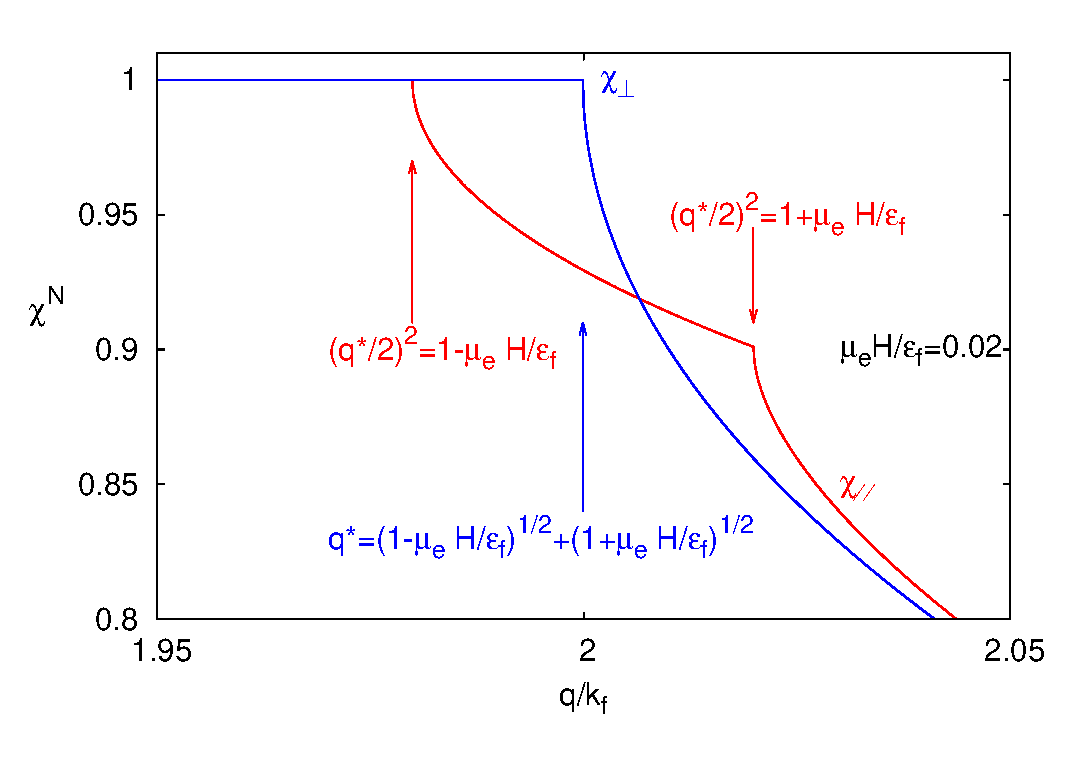
\includegraphics[width=\textwidth]{./figures/chiNormal.eps}
                \caption{The 2D normal state susceptibility has a discontinuity in the first derivative which is split by the field for the parallel component and shifted for the perpendicular component.}
        \end{subfigure}
         \begin{subfigure}[b]{0.23\textwidth}

                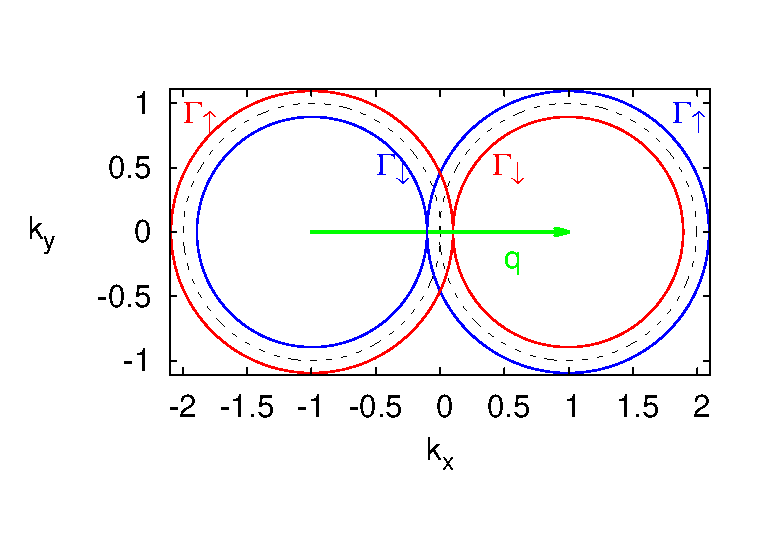
\includegraphics[width=\textwidth]{./figures/SpinPairingxx.eps}
                \caption{The perpendicular component pairs opposite spins. Thus, the paired surfaces are tangent for the same $q^* =\sqrt{1-\mu_e H}+\sqrt{1+\mu_e H}$, and there remains only one discontinuity. }
        \end{subfigure}
         \begin{subfigure}[b]{0.23\textwidth}

                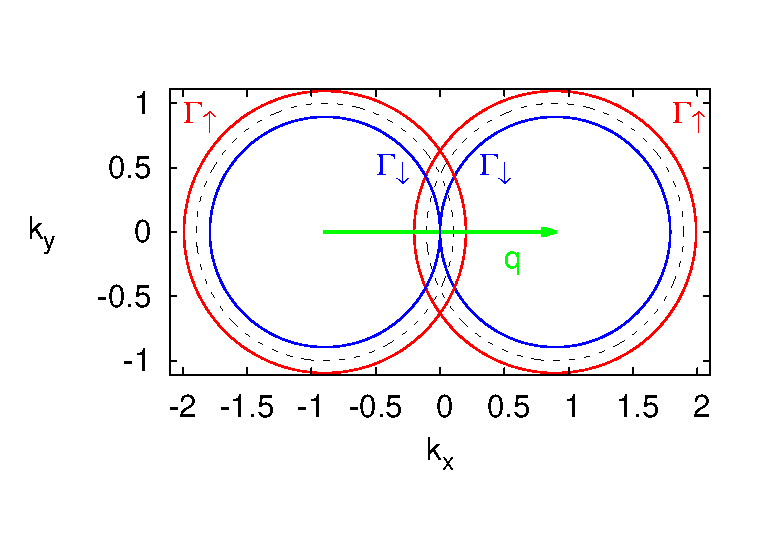
\includegraphics[width=\textwidth]{./figures/SpinPairingzz.eps}
                \caption{The parallel component pairs equal spins. Thus, the spin down surfaces are tangent for a smaller q than the spin up surfaces. Because of this the discontinuity is split into two.}
        \end{subfigure}
 \end{figure}
 
\section{Normal State}
The normal state susceptibility has been studied extensively and reduces to a Lindhard function (equations 4)~\cite{mahan}. For free electrons in a field (excluding orbital effects) the dispersion relation is $\xi_{{\bf k}s}=\frac{k^2}{2m^*}+s\mu_e H-\mu$. At zero temperature the integrand can be done analytically in a two dimensional phase space, with the result given in equations 5. 

\begin{subequations}
\begin{align}
\chi_{\parallel}=-2\mu_e^2\sum\limits_{{\bf k},s} \frac{ f(\epsilon_{{\bf k},s})-f(\epsilon_{{\bf k+q},s})}{ \epsilon_{{\bf k},s}-\epsilon_{{\bf k+q},s}} \\
\chi_{\perp}=-2\mu_e^2\sum\limits_{{\bf k},s} \frac{ f(\epsilon_{{\bf k},s})-f(\epsilon_{{\bf k+q},\bar{s}})}{ \epsilon_{{\bf k},s}-\epsilon_{{\bf k+q},\bar{s}}}
\end{align}
\end{subequations}

\begin{subequations}
{\fontsize{4}{6}\selectfont
\begin{align}
\frac{\chi^N_\parallel(q)}{\chi^N_0}& = \left\{
     \begin{array}{lr}
       1: \quad q < 2\sqrt{1-\mu_e H}\\
       1-\frac{1}{2}\sqrt{1-(\frac{2}{q})^2(1-\mu_e H)}: \quad q \in [2\sqrt{1-\mu_e H},2\sqrt{1+\mu_e H}] \\
       1-\frac{1}{2}\sqrt{1-(\frac{2}{q})^2(1-\mu_e H)}-\frac{1}{2}\sqrt{1-(\frac{2}{q})^2(1+\mu_e H)}:q > 2\sqrt{1+\mu_e H}
     \end{array}
   \right. \\
\frac{\chi^N_\perp(q)}{\chi^N_0} &= \left\{
     \begin{array}{lr}
       1 :\quad q < \sqrt{1-\mu_e H}+\sqrt{1+\mu_e H} \\
       1-\sqrt{1-(\frac{2}{q})^2+(\frac{2\mu_e H}{q^2})^2} : \quad q >\sqrt{1-\mu_e H}+\sqrt{1+\mu_e H}
     \end{array}
   \right.
\end{align}
}
\end{subequations}

The resulting equation(s) 5 have a discontinuity in the first derivitive, the origin of which is the competition between the amount of phase space available to the sum which is defined by the fermi functions, and the term in the denominator, which is proportional to the distance from the origin. For $q<2k_f$ these two balance each other perfectly (as q grows the available phase space grows and the average distance from the origin also increases). For $q>2k_f$ the amount of phase space available is maximized so it can no longer keep up with the average distance from the origin increasing, so the susceptibility begins to fall off. 

When a field is applied to the system the transverse and longitudinal components begin to differentiate themselves due to the way they pair spins (figure 1). The transverse component pairs opposite spins so there is only one critical q at which the available phase space is maximized, $q >\sqrt{1-\mu_e H}+\sqrt{1+\mu_e H}$. The longitudinal component pairs equal spins so there are two critical q's which maximize the phase space for spins up and down respecfully $q = 2\sqrt{1-\mu_e H}$ and $q = 2\sqrt{1+\mu_e H} $.



\section{Superconducting State}
We proceed further into the superconducting state with D-wave symmetry. The inclusion of a Zeeman term in the superconducting Hamiltonian and a nodal order parameter ensures that for high enough fields the Zeeman splitting of the energy levels is enough to overcome the superconducting gap somewhere on the Fermi surface. This becomes critical to the enhancement of the susceptibility becuase with no applied field or for order parameters which are not nodal, the excitation energies $\epsilon_{{\bf k},s}$ are always positive so at zero temperature the fermi functions $f(\epsilon_{{\bf k},s})=0$ everywhere in the phase space and the susceptibility reduces to known results for an s-wave superconductor~\cite{spin_sus}.

Spin up particles (s=-1) provide the necessary condition for $\epsilon_{{\bf k},s}<0$, so the fermi function is zero everywhere except for pockets which open up near the nodes of the order parameter where it is one. This effect also dictates the terms in equation(s) 3 which provide the major contributions. It is those which pair equal spins so that for s=-1, both the $\bf {k+q}/2$ and $\bf{k-q}/2$ fermi surfaces have pockets. We discuss further consequences of this in the results section.
 
The integrals in equations 3 are not analytic by todays methods, however, numerical analysis of the integrand for $\delta \chi_{\alpha}({\bf q})= \chi_{\alpha}({\bf q})^{sc}- \chi_{\alpha}({\bf q})^N$ indicates that value of is less than $(\Delta_{00}/\epsilon_f)^2$ in the majority of phase space and that the main contributions come from regions which are close to the intersections of the two fermi surfaces (figure 3). This is the region where the effects of the phase space pockets brought on by the unconventional order parameter begins to dominate.~\cite{sc_afm_kato,sdw_vortex,sc_afm_ikeda}  


\begin{figure}
\caption{$\delta \chi$ integrands}\label{fig:integrand}
        \centering
        \begin{subfigure}[b]{0.23\textwidth}

                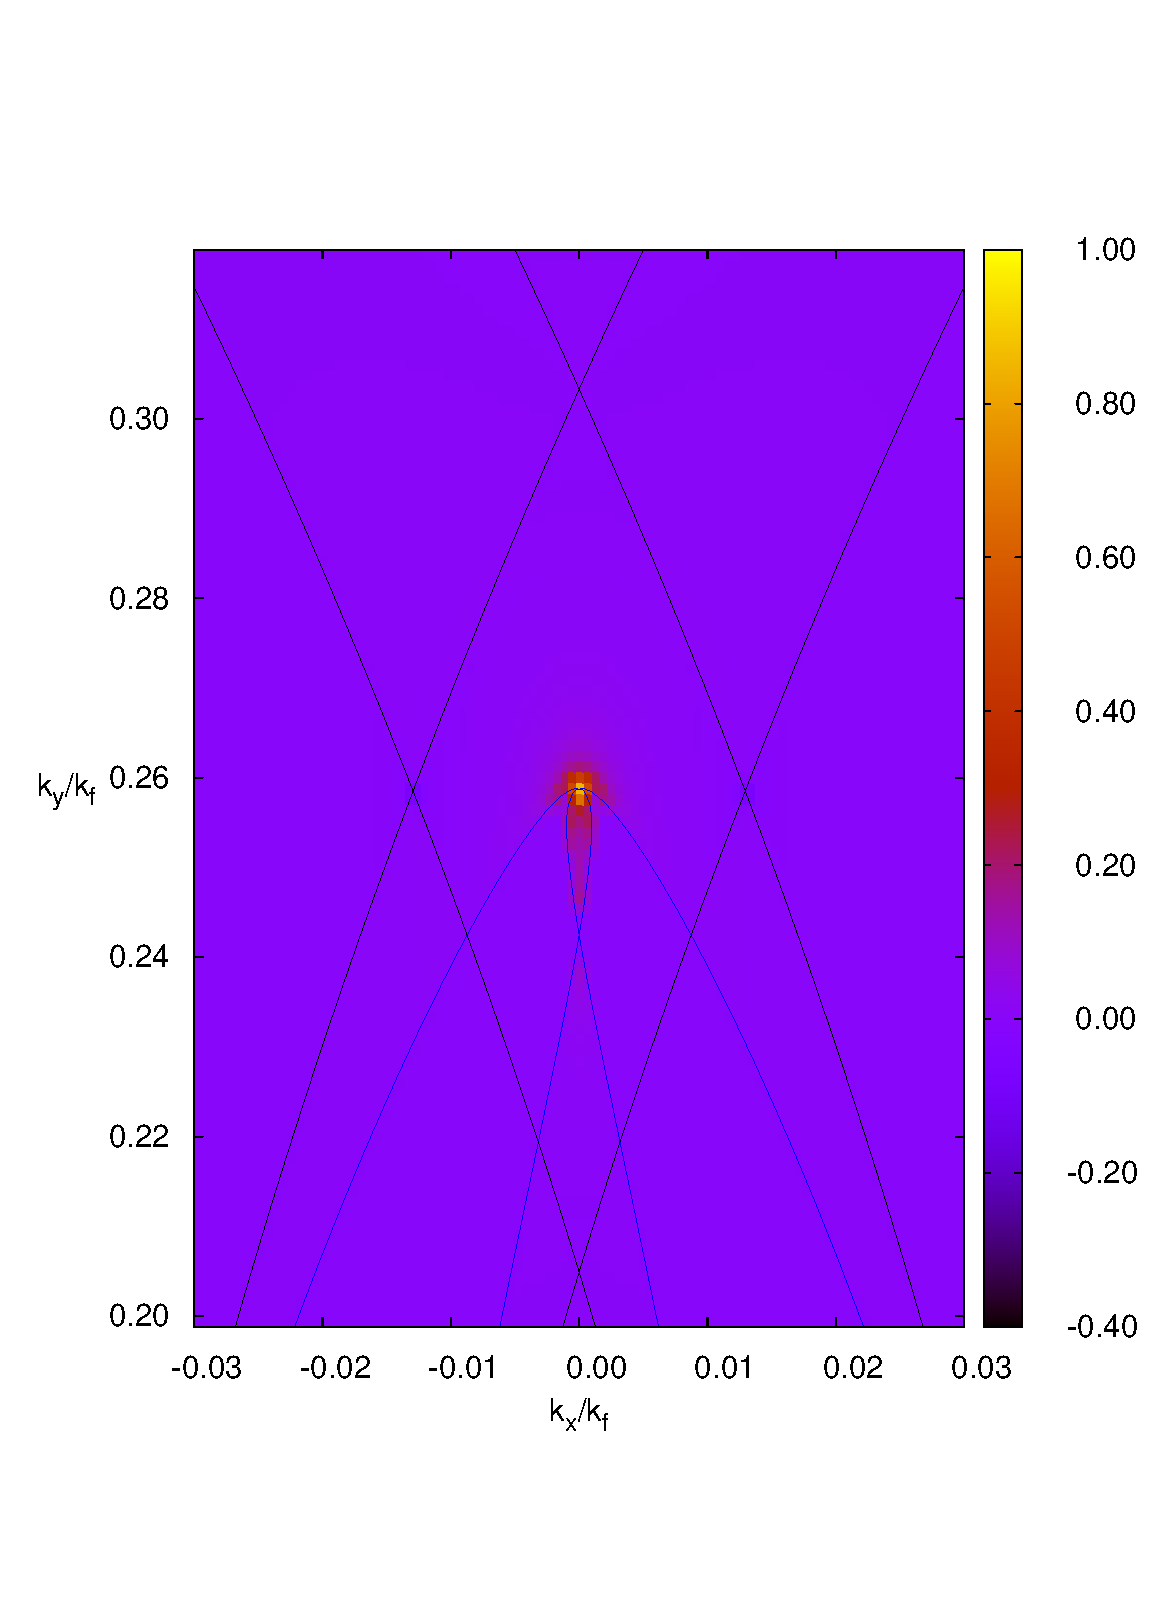
\includegraphics[scale = 0.2]{./figures/difference_perp1.eps}
                \caption{The integrand for the perpendicular component at zero temperature and for the $\bf{q}_{\perp 1}$. The black lines are the zeeman split fermi surfaces for normal electrons and the blue lines are the pockets which open up in the superconducting state.}
        \end{subfigure}
         \begin{subfigure}[b]{0.23\textwidth}

                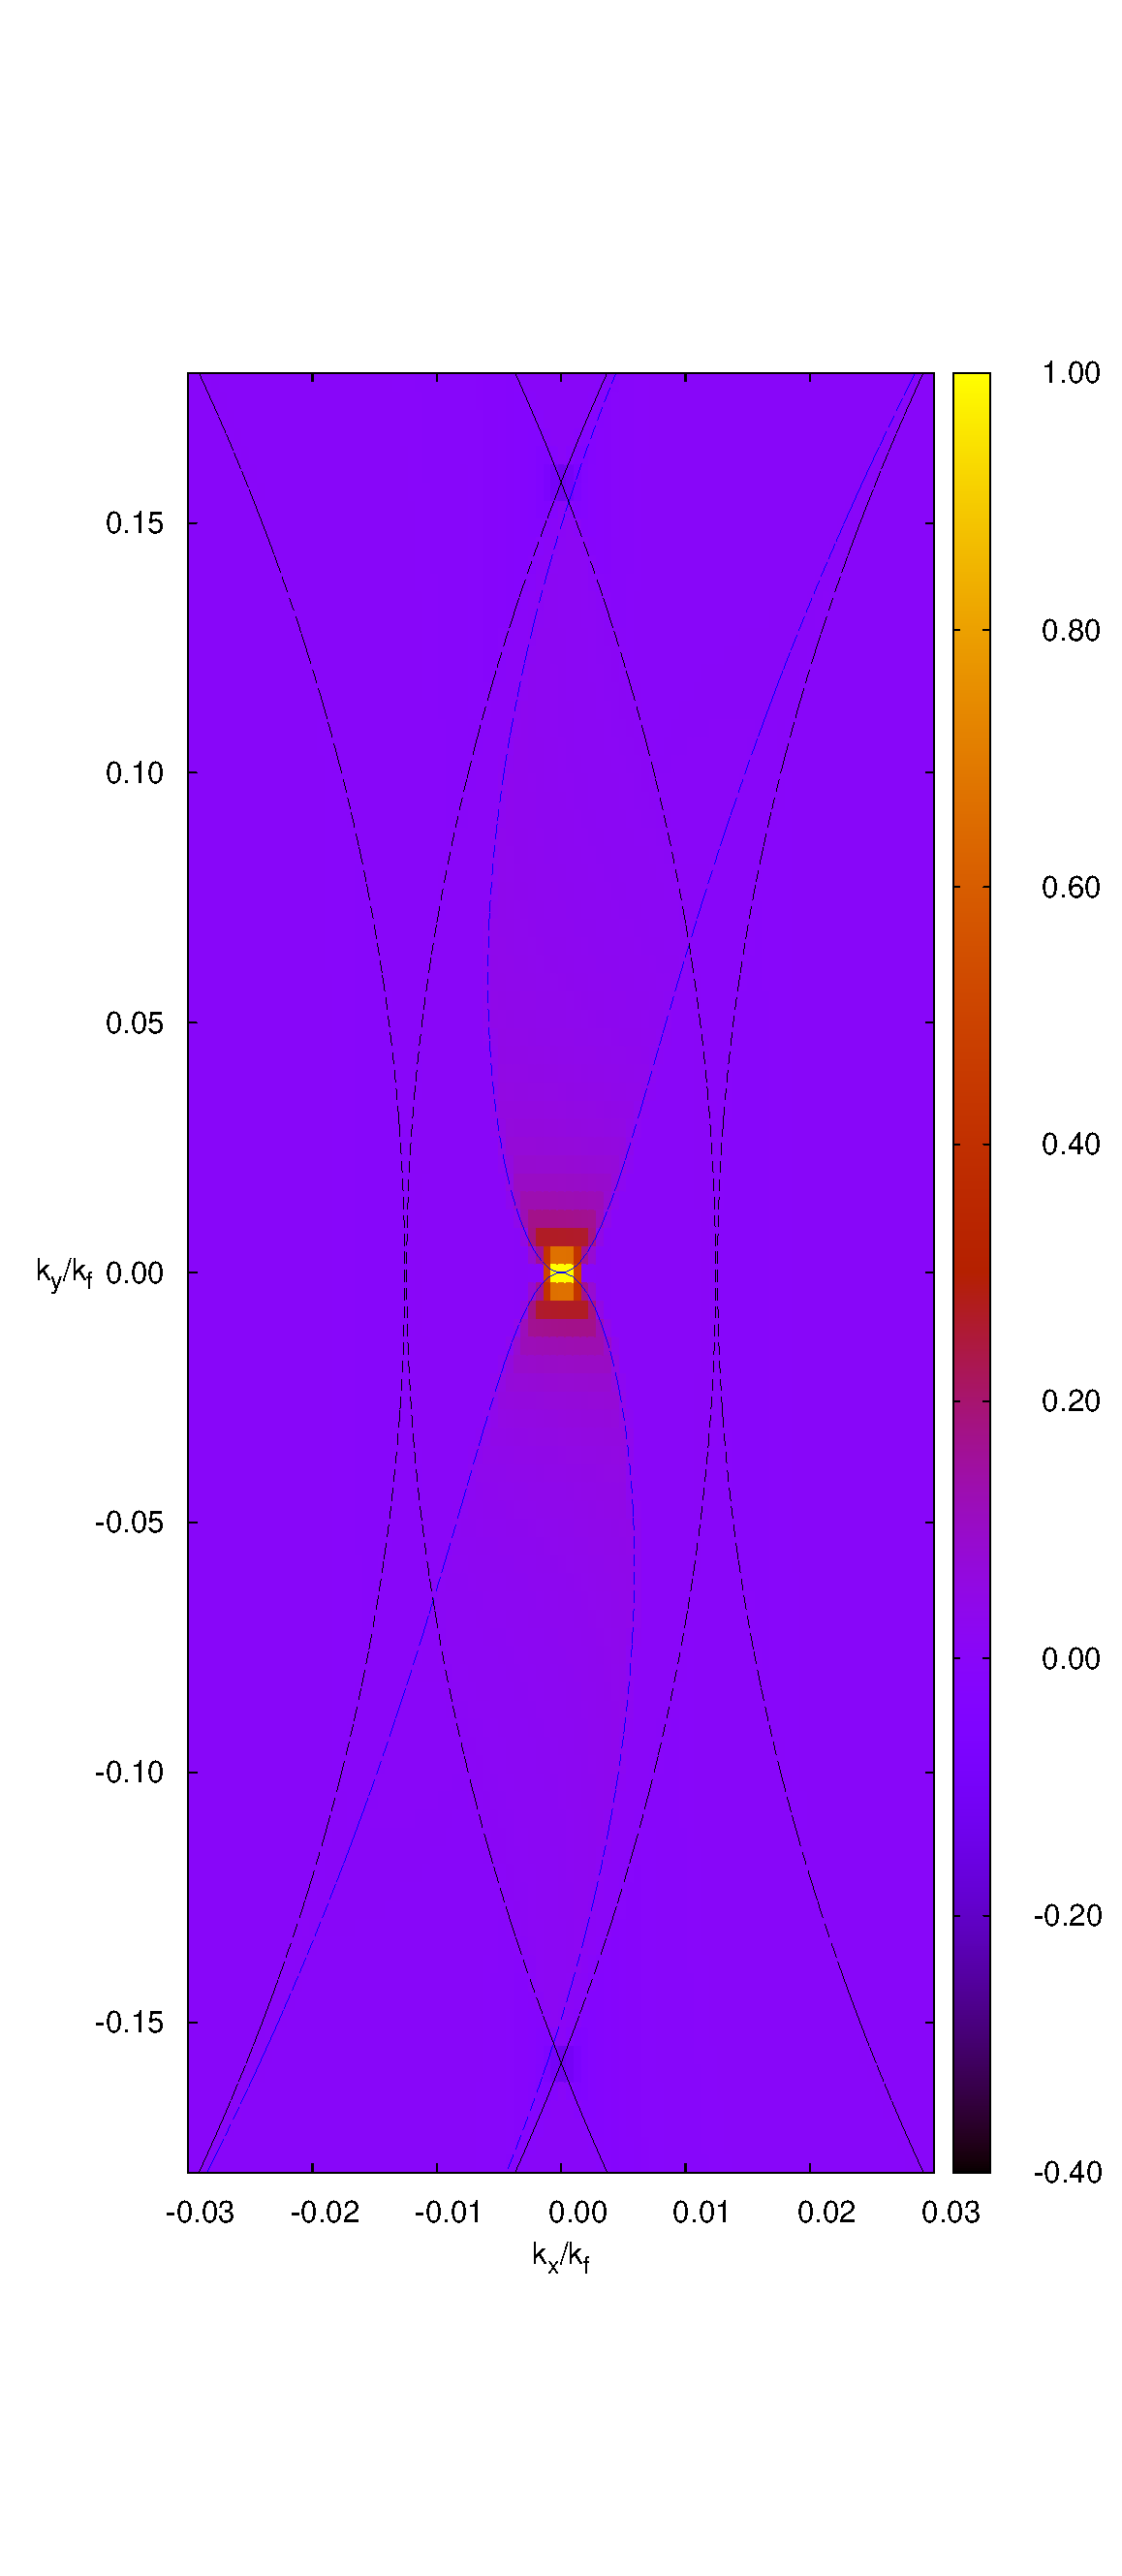
\includegraphics[scale=0.2]{./figures/difference_par1.eps}
                \caption{The integrand for the parallel component at zero temperature and for $\bf{q}_{\parallel 2}$. }
        \end{subfigure}

 \end{figure}

\section{Results}
We further search for the conditions on ${\bf q}$ for which $\chi^{sc}$ is maximized. We find at very low temperatures, that ${\bf q}$'s which connects points where both the quasi-particle energy, $\epsilon_{{\bf k},s}$, and normal state energy, $\xi_{{\bf k}s}$ are zero correspond to maximums in $\chi^{sc}$. This condition gives a zero in the numerator and denominator in equation(s) 3.

For reasons discussed in the previous section, we find that the major contribution to the transverse component comes from the second term in equation 3b. When $\bf q$ is such that it connects points of zero energy excitations both the numerator and denominator go to zero such that the term is still finite, and the phase factor $(u_{k+}v_{k-} -v_{k+}u_{k-})^2$ determines the weight. Because of the subtraction and the positive definite value of $v_k$, this term is maximized for $u_{k+}v_{k-}=-v_{k+}u_{k-}$ which requires $sign(\Delta_{k+})=-sign(\Delta_{k-}$. Thus, the condition on $\bf q^*$ for the transverse component is that it connects the points of zero energy excitations which have opposite sign of $\Delta_{k}$(figure 4a).

Similarly, for the longitudinal component we find the major contributions to come from the first term of equation 3a. Since that term has a plus sign between the two u, v products we require that $\bf q^*$ connect points of zero energy excitations with the same sign of $\Delta_{k}$(figure 4b)



 
  \begin{figure}
\caption{$\bf q^*$}\label{fig:qq}
        \centering
        \begin{subfigure}[b]{0.23\textwidth}

                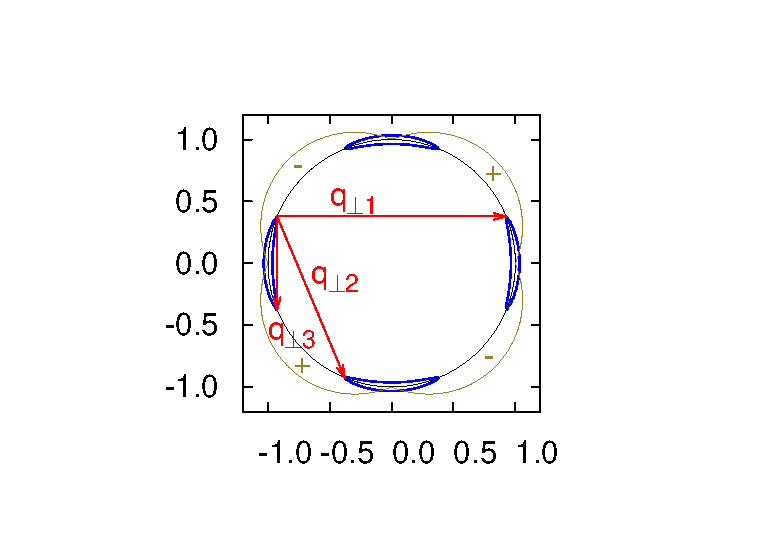
\includegraphics[scale=0.55]{./figures/Bananas_with_q_xx.eps}

        \end{subfigure}
         \begin{subfigure}[b]{0.23\textwidth}

                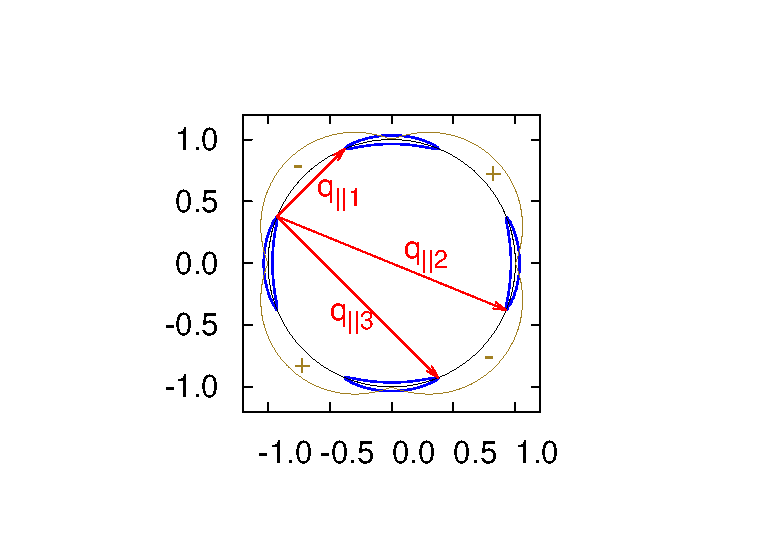
\includegraphics[scale = 0.55]{./figures/Bananas_with_q_zz.eps}

        \end{subfigure}
 \end{figure}



%\begin{figure}
%\caption{$\bf q^*$}\label{fig:qq}
%        \centering
%        \begin{subfigure}[b]{0.23\textwidth}
%
%                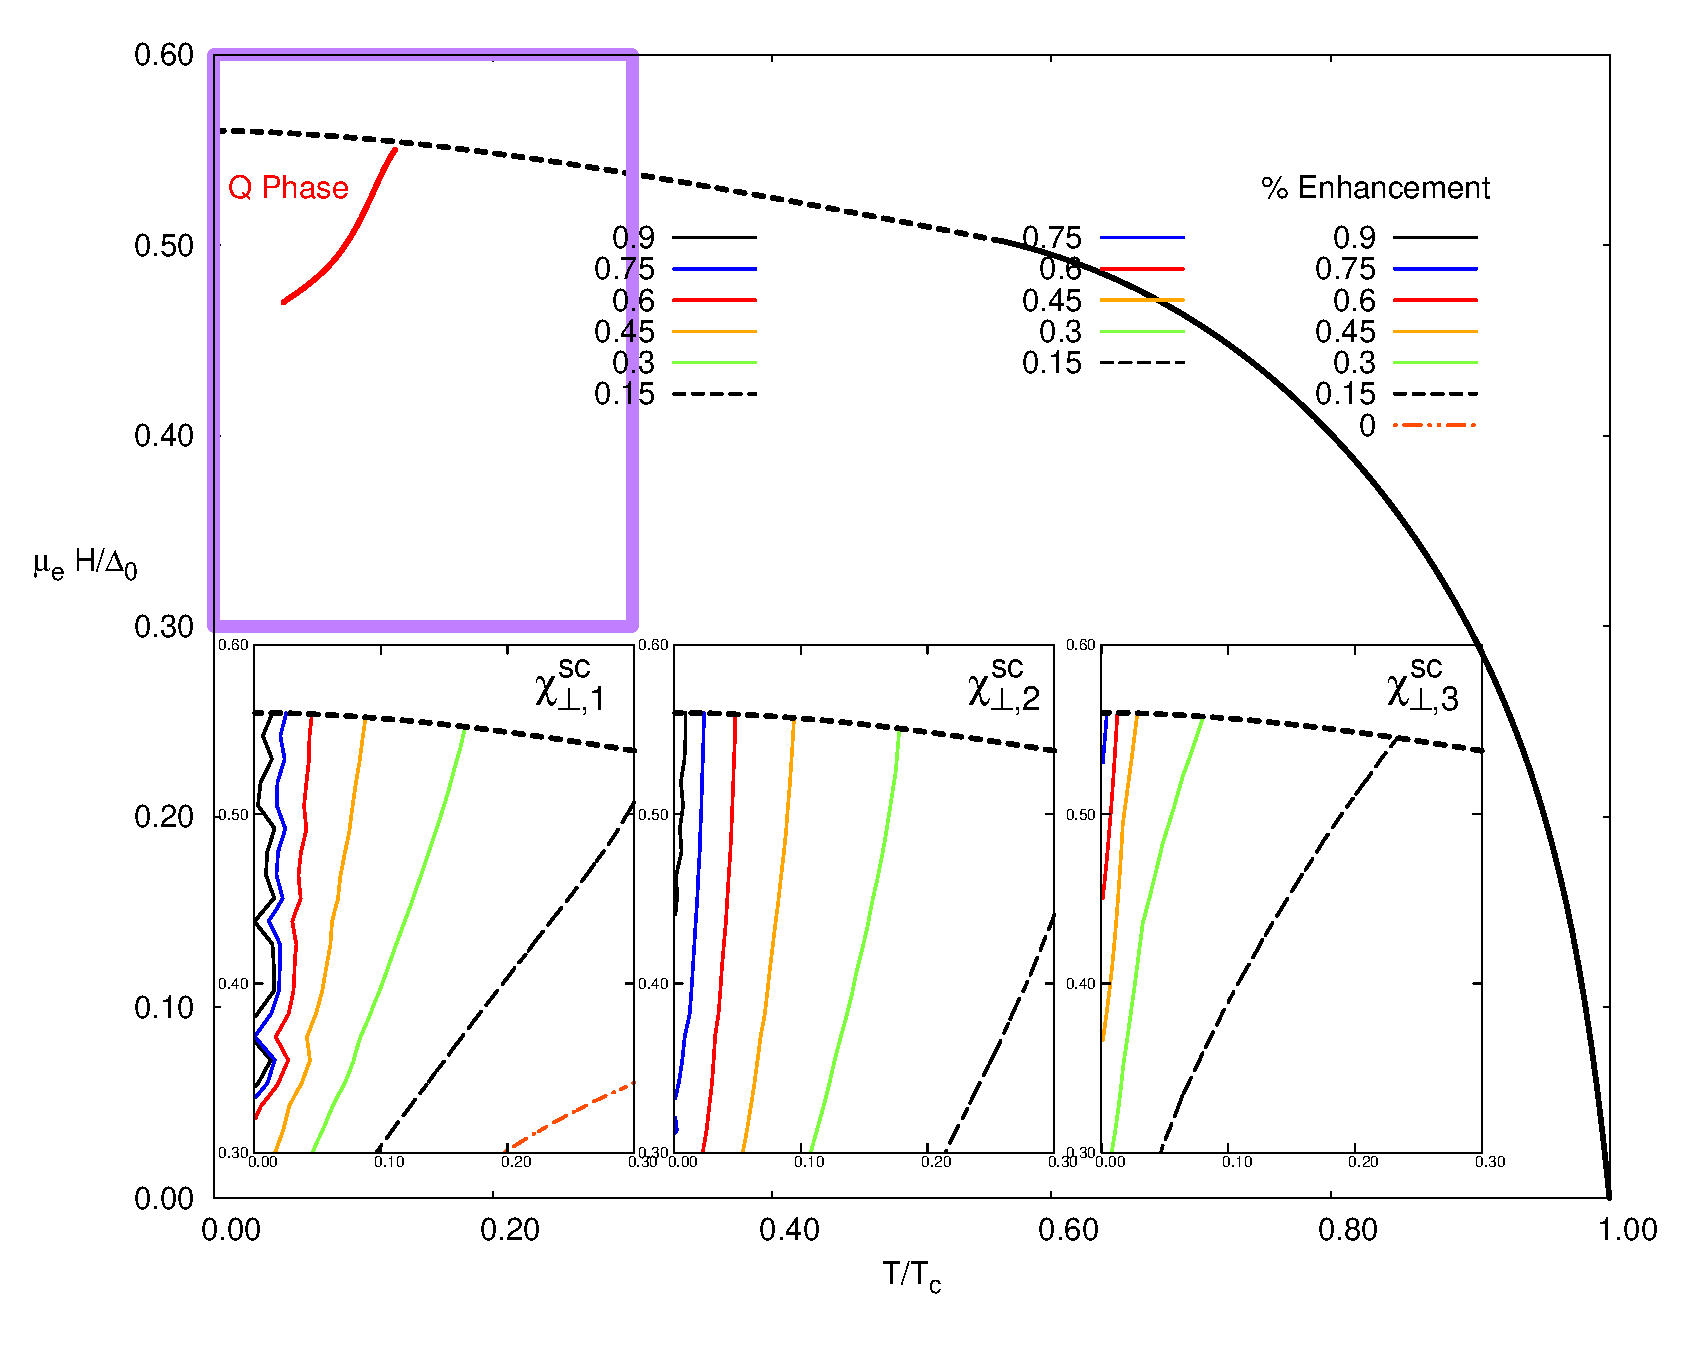
\includegraphics[scale=0.55]{./figures/xx_maxsus_diagram.eps}
%
%        \end{subfigure}
%         \begin{subfigure}[b]{0.23\textwidth}
%
%                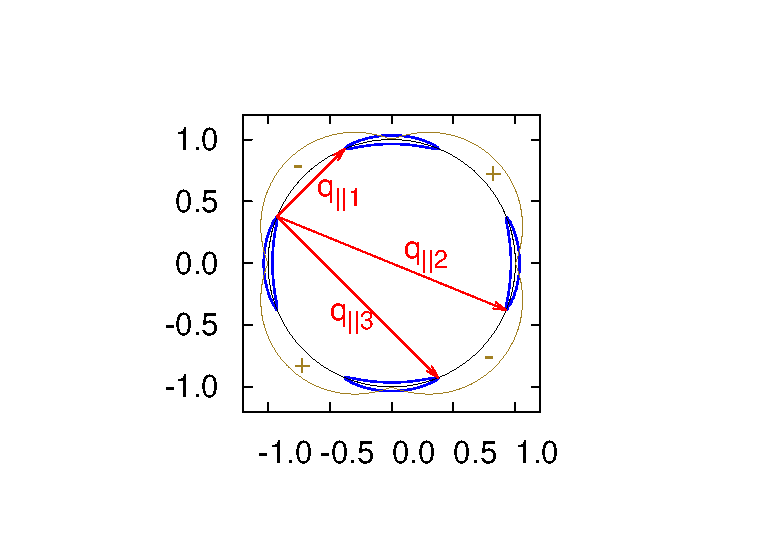
\includegraphics[scale = 0.55]{./figures/Bananas_with_q_zz.eps}
%
%        \end{subfigure}
% \end{figure}
 
 
 
 
%We present results for all the ideal q's in figure 5 for low temperature and fields near $H_{c2}$. 

We present our result in figure 5. At each temperature and field we calculate $\delta \chi$ by numerically integrating near the fermi surface intersections for a range of $\bf q$'s which are near $q_{\parallel 2}$ and $q_{\perp 1}$ respectively.  We then select the maximum $\chi^{sc}=\chi^N+\delta\chi$ in that range of $\bf q$'s.

%\begin{figure}
% 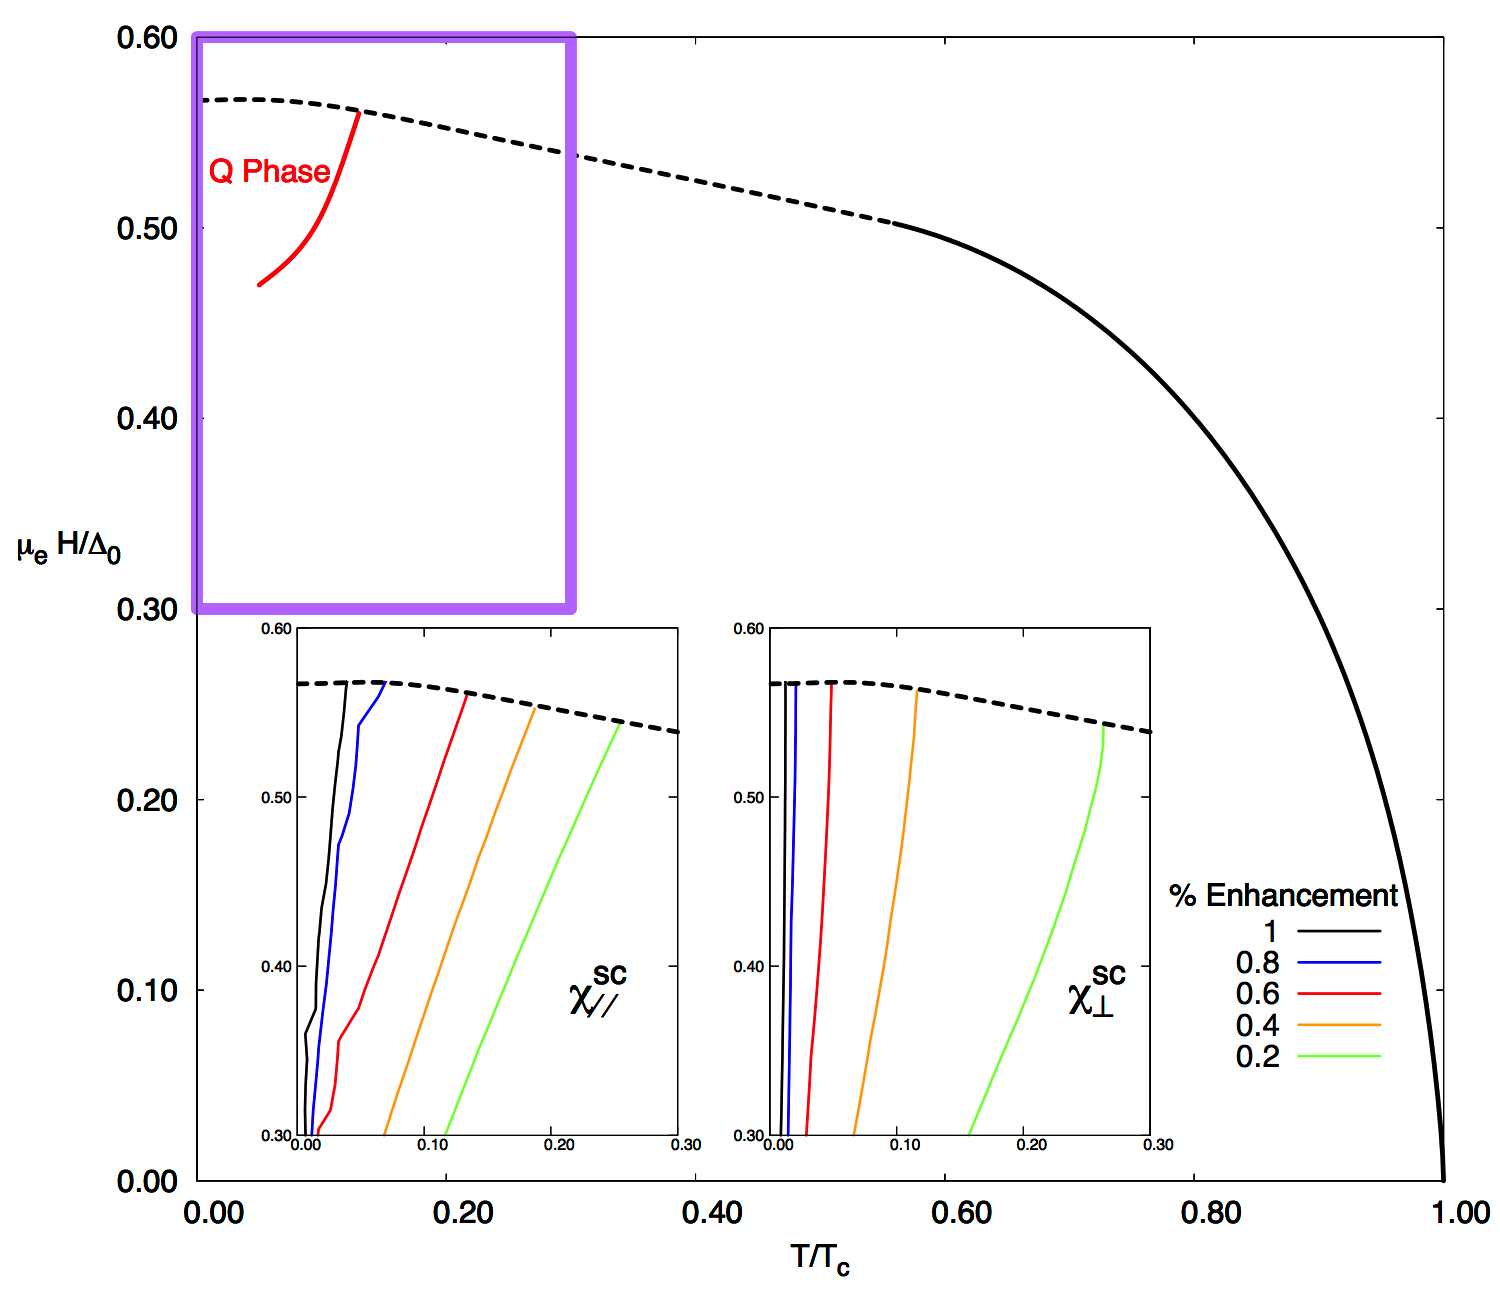
\includegraphics[scale=0.15]{./figures/maxsus_diagram.eps}
% \caption{Phase diagram of CeCoIn$_5$ with insets of the parallel and perpendicular susceptibility enhancement. At each temperature and field we find that maximum susceptibility over a range of $\bf q$ near  $q_{\parallel 2}$ and $q_{\perp 1}$. Figure 7 shows the temperature and field dependence of $\bf q^*$.}
% \end{figure}
 
We believe the behavior of the ideal wave vector ${\bf q}^*(H,T)$ is of particular interest because it provides the possibility of further experimental work which could shed more light on this phenomenon. Figure 6 shows how the ideal wave vector found numerically depends on temperature and field.  As temperature increases the ideal wave vector begins to deviate away from the zero temperature case in such a way that it overlaps the fermi pockets more ($|\bf{q}|$ becomes smaller for both components). 

One interesting feature is shown in figure 6b. The direction of the ideal $\bf q$ for the longitudinal component deviates significantly from the predicted value for higher temperatures and becomes purely nodal for $T>~0.25T_c$. This is deviation is much greater than that of the transverse component. We propose two possible reasons for this result. Firstly, $\chi^N_{\parallel}$ begins to drop off for $|\bf{q}|<2k_f$ (figure 2). Thus, there is a competition between this drop off and the enhancement in $\delta \chi$ which may cause the system to prefer a $\bf q$ which is more nodal for higher temperatures. Secondly, $\bf{q}_{\parallel 2}$ connects the points of zero excitation energy in such a way that the pockets are touching, not overlapping slightly as in the transverse case (figure 3). For finite temperature the edges of these pockets get smeared out and may also cause the system to prefer a more nodal $\bf q$.

 \begin{figure}
\caption{behavior of $\bf q^*$}\label{fig:integrand}
        \centering
        \begin{subfigure}[b]{0.23\textwidth}

                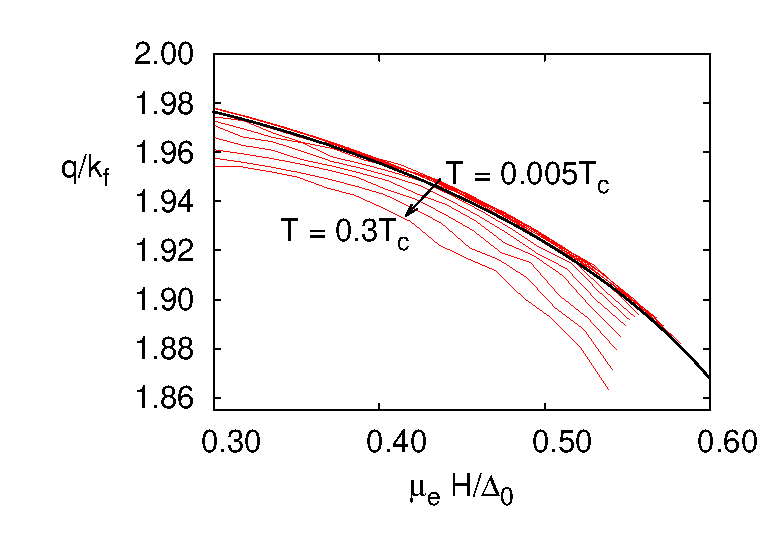
\includegraphics[width=\textwidth]{./figures/max_q_x.eps}
                \caption{The ideal wave vector magnitude for the perpendicular component. $\theta_q$ is always zero for this component and is not plotted here.}
        \end{subfigure}
         \begin{subfigure}[b]{0.23\textwidth}

                \includegraphics[width=\textwidth]{./figures/max_p_z.eps}
                \caption{The ideal wave vector direction for the parallel component. }
        \end{subfigure}

	\begin{subfigure}[b]{0.23\textwidth}

                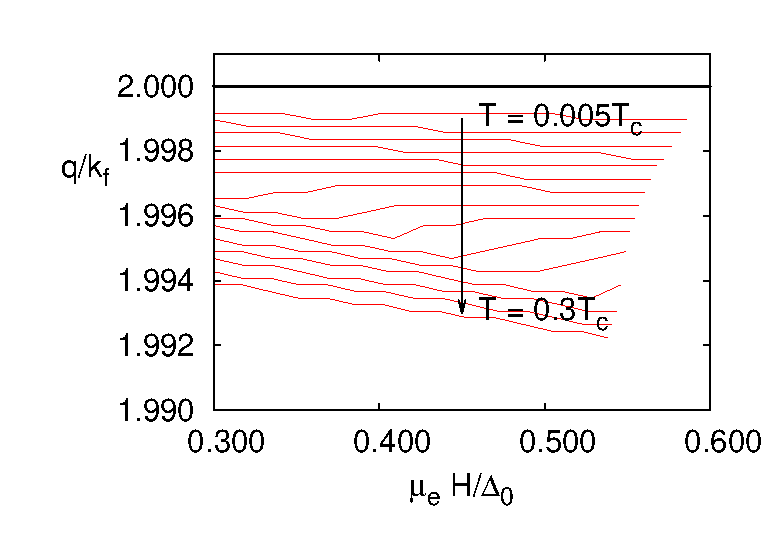
\includegraphics[width=\textwidth]{./figures/max_q_z.eps}
                \caption{The ideal wave vector magnitude for the parallel component.}
        \end{subfigure}
 \end{figure}
 
\section{conclusions}
We find that for certain ordering wave vectors, the superconducting magnetic susceptibility becomes enhanced over the normal state. At zero temperature, these ideal wave vectors connect points on the zero field fermi surface corresponding to zero qusiparticle excitation energy $\epsilon_{{\bf k},s}$ which can only occur for order parameters which become sufficiently small.

Due to the terms in equation 3 which drive this enhancement we can also conclude that the enhancement in $\chi^{sc}_{\perp}$ can only occur for order parameters which are nodal (ie change sign) becuase the ideal $\bf q$'s connect points of zero excitation energy and opposite signs of the order parameter. This contrasts with the longitudinal component which prefers wave vectors which connect regions of the same sign of the order parameter. Thus, the longitudinal componenet may become enhanced for strongly anisotropic superconductors if the order parameter becomes sufficiently small.

We believe that the enhancement of $\chi$ may be enough to establish magnetic order inside the superconducting state. In the case of CeCoIn$_5$ it may also explain the collapse of AMF with superconductivity at H$_{c2}$. This conclusion follows from the equaiton for total susceptibility in terms of the first order expansion and the magnetic interaction(equation 6). If a normal state material were to have a susceptibility and magnetic interaction such that $1-J_{\alpha\beta} \chi_{\alpha\beta}<<1$, then a small enhancement of $\chi_{\alpha\beta}$ could be sufficent to induce magnetic order. In the case of itinerant electrons, this order would be in the form of a spin density wave (SDW). The origins of the magnetic interaction $J_{\alpha\beta}$ are not discussed here, but may be from coupling to the localized magnetic moments of the Ce atoms, (RKKY interaction CITE) or by some other mechanism. Our findings indicate that under certain conditions $\chi_{\alpha\beta}$ in the superconducting state can indeed increase over the normal state value for certain ideal ordering wave vectors, providing the necessary condition for a SDW.

\begin{align}
\chi^{total}_{\alpha\beta}=\frac{\chi_{\alpha\beta}}{1-J_{\alpha\beta} \chi_{\alpha\beta}}
\end{align}




%One key feature of the critical values at which $\chi^{sc}$ is maximized is that $q^*$ is a decreasing function of applied field. FFLO state calculations also have this feature. However, experimental results in CeCoIn$_5$ show a small increase in $q^*$ with increasing field.\cite{cecoin5_Kenzelmann2} This fact is often ignored in many theories, but may provide a deeper insight into the phenomenon which is not yet understood.\cite{spin_sus_dyn,sdw_vortex,sc_afm_ikeda,sc_afm_kato,mag_afm_fflo_sigrist,sc_sdw_anton}

\bibliography{mybib}{}
\bibliographystyle{plain}
\end{document}